\documentclass[border=15pt, tikz]{standalone}
\usepackage[T1]{fontenc}
\usepackage[utf8]{inputenc}
\usepackage{tikz}
\usetikzlibrary{positioning, arrows.meta, decorations.pathreplacing, calc, fit}
\definecolor{clrattention}{HTML}{45B7D1}
\definecolor{clrattention_alt}{HTML}{96E6F0}
\definecolor{clrffn}{HTML}{F97068}
\definecolor{clrnorm}{HTML}{FFD93D}
\definecolor{clrembed}{HTML}{6BCB77}
\definecolor{clrresidual}{HTML}{4D96FF}
\definecolor{clroutput}{HTML}{C084FC}
\definecolor{clrspectral}{HTML}{22D3EE}
\definecolor{clrphysics}{HTML}{FB923C}
\definecolor{clrborder}{HTML}{334155}
\definecolor{clrtext}{HTML}{1E293B}
\definecolor{clrgroup_frame}{HTML}{94A3B8}
\definecolor{clrgroup_fill}{HTML}{F1F5F9}
\begin{document}
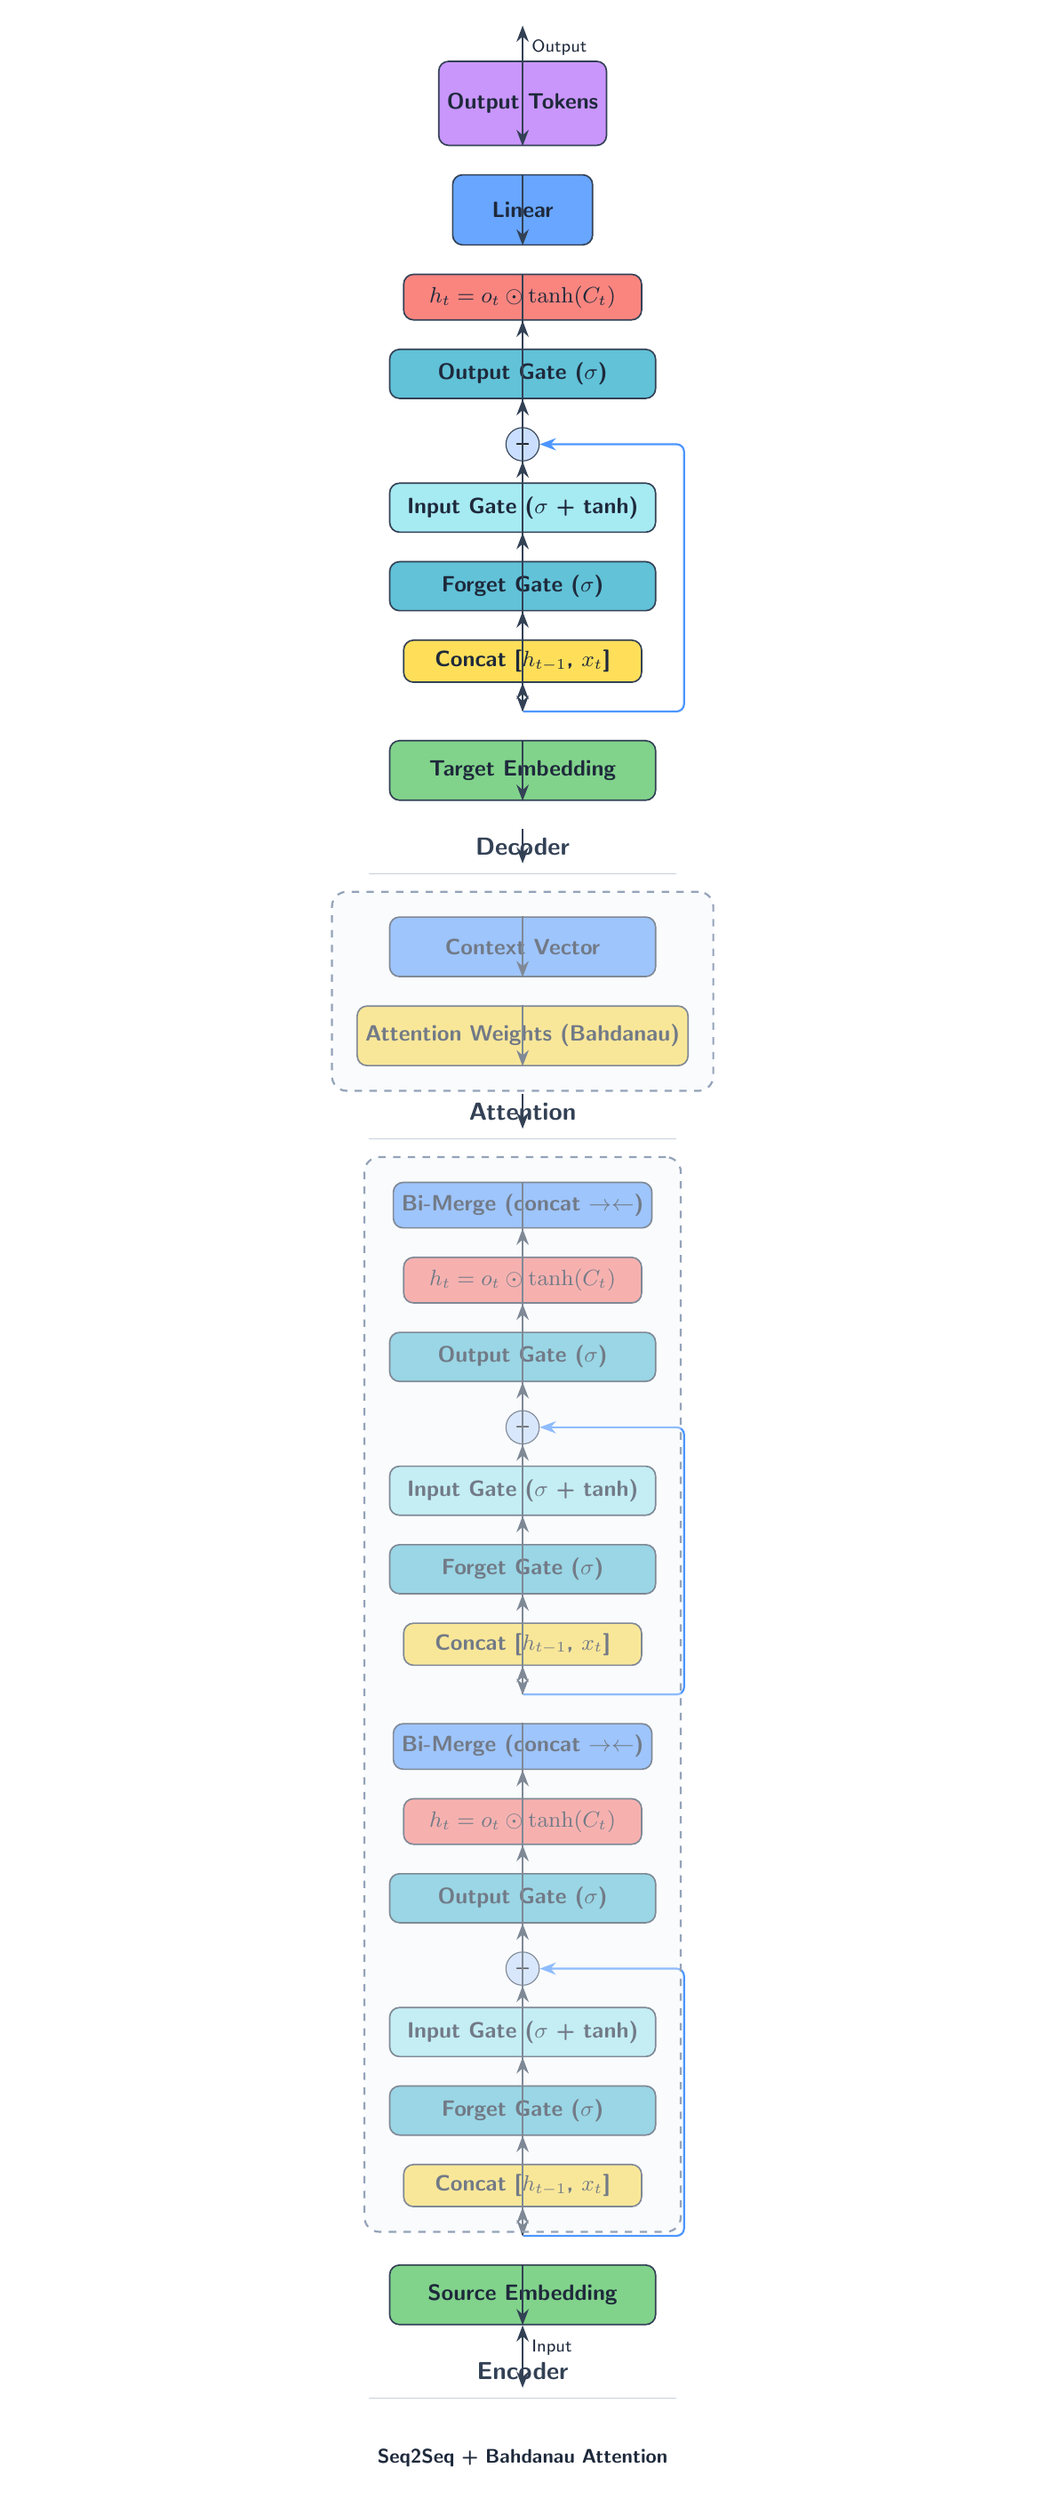
\begin{tikzpicture}[
    >=Stealth,
    every node/.style={font=\sffamily},
    block/.style={draw=clrborder, rounded corners=4pt, minimum width=3.8cm,
                  minimum height=0.85cm, font=\sffamily\small\bfseries,
                  text=clrtext, line width=0.6pt},
    arrow/.style={->, thick, color=clrborder, line width=0.8pt},
    skiparrow/.style={->, thick, color=clrresidual, line width=0.8pt, rounded corners=3pt},
    label/.style={font=\sffamily\scriptsize, text=clrtext},
    subtitle/.style={font=\sffamily\footnotesize, text=clrtext},
]
\node[inner sep=0, minimum height=0] (n_1_rule) at (0,0) {};
\draw[color=clrgroup_frame!50, line width=0.4pt] ([xshift=-2.2cm]n_1_rule.center) -- ([xshift=2.2cm]n_1_rule.center);
\node[above=4pt of n_1_rule, font=\sffamily\normalsize\bfseries, text=clrborder] (n_1) {Encoder};
\node[block, fill=clrembed!85, minimum width=3.8cm, minimum height=0.85cm, text=clrtext, above=0.4cm of n_1] (n_2) {Source Embedding};
\node[inner sep=0, minimum size=0, above=0.4cm of n_2] (res_entry_3) {};
\node[block, fill=clrnorm!85, minimum width=3.4cm, minimum height=0.6cm, text=clrtext, above=0.4cm of res_entry_3] (n_4) {Concat [$h_{t-1}$, $x_t$]};
\node[block, fill=clrattention!85, minimum width=3.8cm, minimum height=0.7cm, text=clrtext, above=0.4cm of n_4] (n_5) {Forget Gate ($\sigma$)};
\node[block, fill=clrattention_alt!85, minimum width=3.8cm, minimum height=0.7cm, text=clrtext, above=0.4cm of n_5] (n_6) {Input Gate ($\sigma$ + tanh)};
\node[circle, draw=clrborder, fill=clrresidual!30, inner sep=2pt, font=\sffamily\scriptsize\bfseries, above=0.3cm of n_6] (add_7) {+};
\node[block, fill=clrattention!85, minimum width=3.8cm, minimum height=0.7cm, text=clrtext, above=0.4cm of add_7] (n_8) {Output Gate ($\sigma$)};
\node[block, fill=clrffn!85, minimum width=3.4cm, minimum height=0.65cm, text=clrtext, above=0.4cm of n_8] (n_9) {$h_t = o_t \odot \tanh(C_t)$};
\node[block, fill=clrresidual!85, minimum width=3.4cm, minimum height=0.65cm, text=clrtext, above=0.4cm of n_9] (n_10) {Bi-Merge (concat $\rightarrow \leftarrow$)};
\node[inner sep=0, minimum size=0, above=0.4cm of n_10] (res_entry_11) {};
\node[block, fill=clrnorm!85, minimum width=3.4cm, minimum height=0.6cm, text=clrtext, above=0.4cm of res_entry_11] (n_12) {Concat [$h_{t-1}$, $x_t$]};
\node[block, fill=clrattention!85, minimum width=3.8cm, minimum height=0.7cm, text=clrtext, above=0.4cm of n_12] (n_13) {Forget Gate ($\sigma$)};
\node[block, fill=clrattention_alt!85, minimum width=3.8cm, minimum height=0.7cm, text=clrtext, above=0.4cm of n_13] (n_14) {Input Gate ($\sigma$ + tanh)};
\node[circle, draw=clrborder, fill=clrresidual!30, inner sep=2pt, font=\sffamily\scriptsize\bfseries, above=0.3cm of n_14] (add_15) {+};
\node[block, fill=clrattention!85, minimum width=3.8cm, minimum height=0.7cm, text=clrtext, above=0.4cm of add_15] (n_16) {Output Gate ($\sigma$)};
\node[block, fill=clrffn!85, minimum width=3.4cm, minimum height=0.65cm, text=clrtext, above=0.4cm of n_16] (n_17) {$h_t = o_t \odot \tanh(C_t)$};
\node[block, fill=clrresidual!85, minimum width=3.4cm, minimum height=0.65cm, text=clrtext, above=0.4cm of n_17] (n_18) {Bi-Merge (concat $\rightarrow \leftarrow$)};
\node[above=0.6cm of n_18, inner sep=0, minimum height=0] (n_19_rule) {};
\draw[color=clrgroup_frame!50, line width=0.4pt] ([xshift=-2.2cm]n_19_rule.center) -- ([xshift=2.2cm]n_19_rule.center);
\node[above=4pt of n_19_rule, font=\sffamily\normalsize\bfseries, text=clrborder] (n_19) {Attention};
\node[block, fill=clrnorm!85, minimum width=3.8cm, minimum height=0.85cm, text=clrtext, above=0.4cm of n_19] (n_20) {Attention Weights (Bahdanau)};
\node[block, fill=clrresidual!85, minimum width=3.8cm, minimum height=0.85cm, text=clrtext, above=0.4cm of n_20] (n_21) {Context Vector};
\node[above=0.6cm of n_21, inner sep=0, minimum height=0] (n_22_rule) {};
\draw[color=clrgroup_frame!50, line width=0.4pt] ([xshift=-2.2cm]n_22_rule.center) -- ([xshift=2.2cm]n_22_rule.center);
\node[above=4pt of n_22_rule, font=\sffamily\normalsize\bfseries, text=clrborder] (n_22) {Decoder};
\node[block, fill=clrembed!85, minimum width=3.8cm, minimum height=0.85cm, text=clrtext, above=0.4cm of n_22] (n_23) {Target Embedding};
\node[inner sep=0, minimum size=0, above=0.4cm of n_23] (res_entry_24) {};
\node[block, fill=clrnorm!85, minimum width=3.4cm, minimum height=0.6cm, text=clrtext, above=0.4cm of res_entry_24] (n_25) {Concat [$h_{t-1}$, $x_t$]};
\node[block, fill=clrattention!85, minimum width=3.8cm, minimum height=0.7cm, text=clrtext, above=0.4cm of n_25] (n_26) {Forget Gate ($\sigma$)};
\node[block, fill=clrattention_alt!85, minimum width=3.8cm, minimum height=0.7cm, text=clrtext, above=0.4cm of n_26] (n_27) {Input Gate ($\sigma$ + tanh)};
\node[circle, draw=clrborder, fill=clrresidual!30, inner sep=2pt, font=\sffamily\scriptsize\bfseries, above=0.3cm of n_27] (add_28) {+};
\node[block, fill=clrattention!85, minimum width=3.8cm, minimum height=0.7cm, text=clrtext, above=0.4cm of add_28] (n_29) {Output Gate ($\sigma$)};
\node[block, fill=clrffn!85, minimum width=3.4cm, minimum height=0.65cm, text=clrtext, above=0.4cm of n_29] (n_30) {$h_t = o_t \odot \tanh(C_t)$};
\node[block, fill=clrresidual!85, minimum width=2.0cm, minimum height=1.0cm, text=clrtext, above=0.4cm of n_30] (n_31) {Linear};
\node[block, fill=clroutput!85, minimum width=2.0cm, minimum height=1.2cm, text=clrtext, above=0.4cm of n_31] (n_32) {Output Tokens};
\draw[arrow] (n_1.north) -- (n_1.south);
\draw[arrow] (n_2.north) -- (n_2.south);
\draw[arrow] (n_4.north) -- (n_5.south);
\draw[arrow] (n_5.north) -- (n_6.south);
\draw[arrow] (res_entry_3.north) -- (n_4.south);
\draw[arrow] (n_6.north) -- (add_7.south);
\draw[skiparrow] (res_entry_3.east) -- ++(2.3,0) |- (add_7.east);
\draw[arrow] (add_7.north) -- (n_8.south);
\draw[arrow] (n_8.north) -- (n_9.south);
\draw[arrow] (n_9.north) -- (n_10.south);
\draw[arrow] (n_10.north) -- (res_entry_3.south);
\draw[arrow] (n_12.north) -- (n_13.south);
\draw[arrow] (n_13.north) -- (n_14.south);
\draw[arrow] (res_entry_11.north) -- (n_12.south);
\draw[arrow] (n_14.north) -- (add_15.south);
\draw[skiparrow] (res_entry_11.east) -- ++(2.3,0) |- (add_15.east);
\draw[arrow] (add_15.north) -- (n_16.south);
\draw[arrow] (n_16.north) -- (n_17.south);
\draw[arrow] (n_17.north) -- (n_18.south);
\draw[arrow] (n_18.north) -- (res_entry_11.south);
\draw[arrow] (n_19.north) -- (n_19.south);
\draw[arrow] (n_20.north) -- (n_20.south);
\draw[arrow] (n_21.north) -- (n_21.south);
\draw[arrow] (n_22.north) -- (n_22.south);
\draw[arrow] (n_23.north) -- (n_23.south);
\draw[arrow] (n_25.north) -- (n_26.south);
\draw[arrow] (n_26.north) -- (n_27.south);
\draw[arrow] (res_entry_24.north) -- (n_25.south);
\draw[arrow] (n_27.north) -- (add_28.south);
\draw[skiparrow] (res_entry_24.east) -- ++(2.3,0) |- (add_28.east);
\draw[arrow] (add_28.north) -- (n_29.south);
\draw[arrow] (n_29.north) -- (n_30.south);
\draw[arrow] (n_30.north) -- (res_entry_24.south);
\draw[arrow] (n_31.north) -- (n_31.south);
\draw[arrow] (n_32.north) -- (n_32.south);
\draw[arrow] (n_2.south) ++ (0,-0.5) -- node[right, yshift=-2pt, font=\sffamily\scriptsize, text=clrtext] {Input} (n_2.south);
\draw[arrow] (n_32.north) -- node[right, yshift=-2pt, font=\sffamily\scriptsize, text=clrtext] {Output} ++ (0,0.5);
\node[draw=clrgroup_frame, rounded corners=6pt, dashed, line width=0.8pt, fill=clrgroup_fill, fill opacity=0.4, inner sep=0.35cm, fit=(n_4) (n_5) (n_6) (n_8) (n_9) (n_10) (n_12) (n_13) (n_14) (n_16) (n_17) (n_18)] (g_0) {};
\node[draw=clrgroup_frame, rounded corners=6pt, dashed, line width=0.8pt, fill=clrgroup_fill, fill opacity=0.4, inner sep=0.35cm, fit=(n_20) (n_21)] (g_1) {};
\node[below=0.6cm of current bounding box.south, subtitle, text width=14cm, align=center] {\textbf{Seq2Seq + Bahdanau Attention}};
\end{tikzpicture}
\end{document}
